\Class{Bard}
{Some people think a club can solve any problem. Unless you're a half-giant, there are more sophisticated ways of settling a disagreement.}{Cabal, half-elven bard}

From the shadowy corners of Athas' most disreputable places hails the bard. Like their counterparts in other fantasy worlds, Athasian bards are the unquestioned masters of oral tradition and forgotten lore, but rather than sharing their lore with whoever will listen, Athasian bards guard their secrets as jealously as the sorcerer-kings harbor their water and iron. Athasian bards may sell information to the highest bidder; they peddle their services and the fruits of their knowledge, but trade secrets are what give bards an edge on the uninitiated. Bards would rather die than reveal these secrets.

Meeting a bard can be an uneasy encounter, since one never knows how the bard has chosen to devote his multiple talents. Some bards master the art of making poisons, and survive by selling these poisons and their antidotes for those who have coin to pay. Some bards master the art of entertainment, using their performances to amuse nobles and templars and gain wealth. Some become assassins, mixing their knowledge of poison and stealth to become hired hands. Bards' unique position in the Athasian society means they often overhear conversations between high-ranking templars or nobles, or they may have treated an injured person that prefers to remain anonymous. Respectable folk despise them; the powerful fear them; but in the Athasian cities, everyone eventually comes to need their services.

\WarriorTable[b{0.8cm} b{2.6cm} Z{1.4cm} Z{1.4cm} Z{1.4cm} X]{The Bard}{
1 & +0 & +2 & +2 & +2 & Bardic music, bardic knowledge, smuggler, countersong, fascinate, inspire courage +1\\
2 & +1 & +3 & +3 & +3 & Poison use, streetsmart\\
3 & +2 & +3 & +3 & +3 & Inspire competence, quick draw\\
4 & +3 & +4 & +4 & +4 & Trade secret\\
5 & +3 & +4 & +4 & +4 & Mental resistance\\
6 & +4 & +5 & +5 & +5 & Improved poison use, suggestion, quick thinking +2\\
7 & +5 & +5 & +5 & +5 & Chance 1/day\\
8 & +6/+1 & +6 & +6 & +6 & Inspire courage +2, trade secret\\
9 & +6/+1 & +6 & +6 & +6 & Inspire greatness, speed reactions\\
10 & +7/+2 & +7 & +7 & +7 & Slippery mind\\
11 & +8/+3 & +7 & +7 & +7 & Quick thinking +4\\
12 & +9/+4 & +8 & +8 & +8 & Song of freedom, trade secret\\
13 & +9/+4 & +8 & +8 & +8 &  \\
14 & +10/+5 & +9 & +9 & +9 & Chance 2/day, inspire courage +3\\
15 & +11/+6/+1 & +9 & +9 & +9 & Defensive roll, inspire heroics\\
16 & +12/+7/+2 & +10 & +10 & +10 & Quick thinking +6, trade secret\\
17 & +12/+7/+2 & +10 & +10 & +10 & Awareness \\
18 & +13/+8/+3 & +11 & +11 & +11 & Mass suggestion, mindblank\\
19 & +14/+9/+4 & +11 & +11 & +11 &  \\
20 & +15/+10/+5 & +12 & +12 & +12 & Inspire courage +4, trade secret
}

\begin{figure}[t!]
\centering
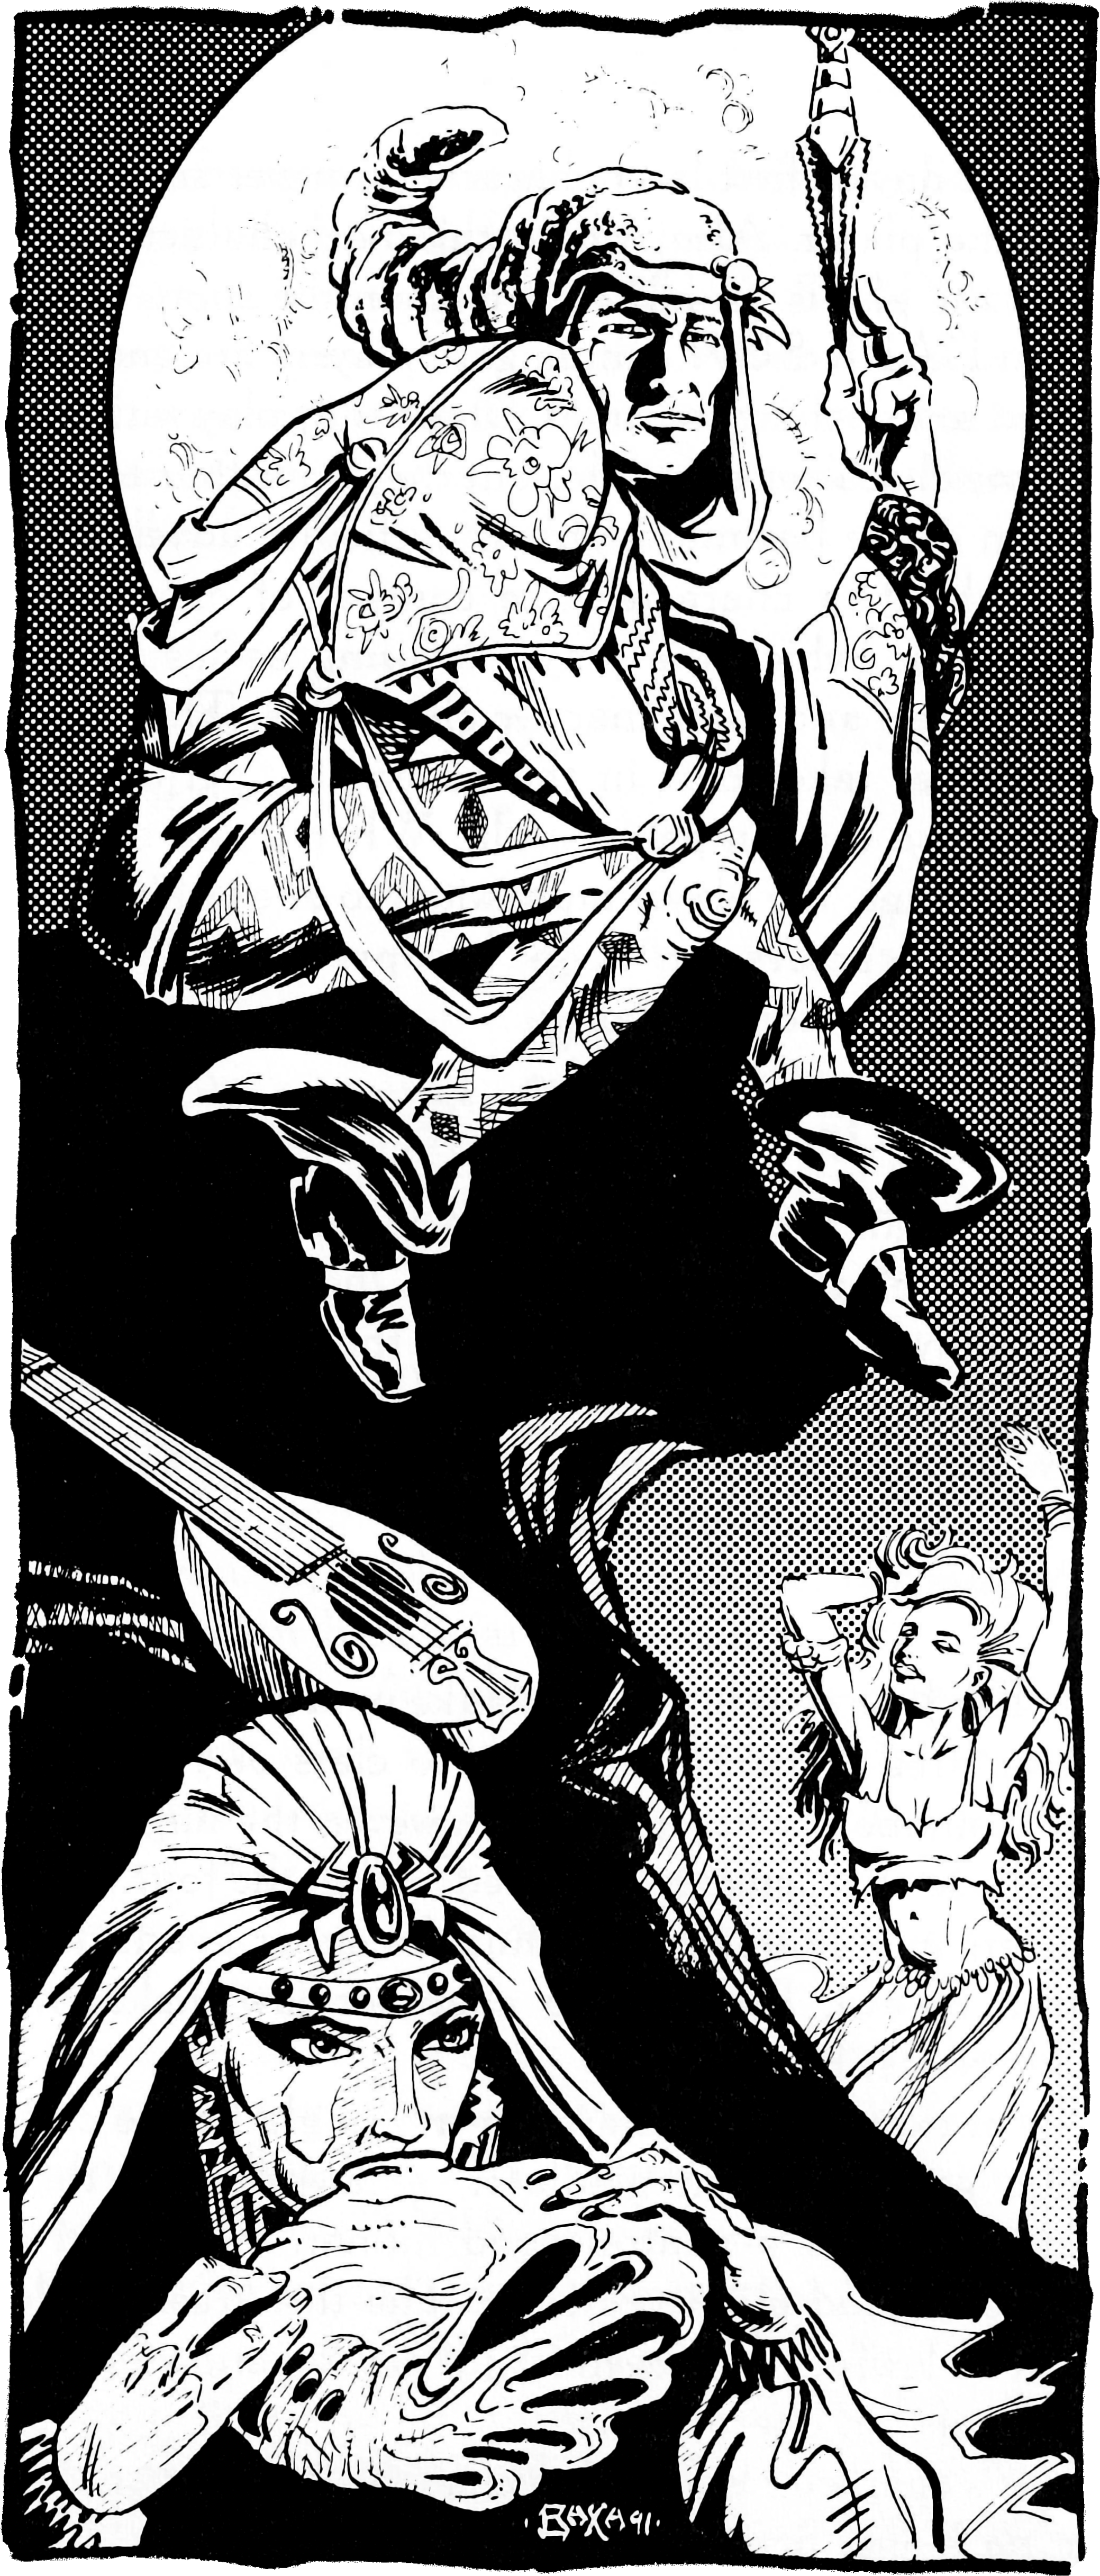
\includegraphics[width=\columnwidth]{images/bard-1.png}
\par\textit{\small\textcopyright Wizards of the Coast, 2020.}
\end{figure}

\subsection{Making a Bard}
Bards receive numerous abilities they can use to survive. Many become masters of poisons, selling their illegal substances to anyone. Alone of the classes, bards hold the secrets of alchemy, creating fiery concoctions and mysterious mixes. Bards are master smugglers, selling spell components and other illegal items in the Bard's Quarters of the city-states. All bards, however, have some degree of entertainment skill. The songs of most bards can dazzle a crowd, or incite them to riot. Bards tend to learn to play a variety of instruments, or recite poetry or old legends by campfire. They can be acrobats, performing dazzling displays of physical prowess. They are often called upon as sources of information.

\textbf{Abilities:} Charisma is the most important ability for a bard, because many of their abilities and skills are affected by it. A high Dexterity improves the bard's defensive ability. Intelligence is also important because it bolster the numbers of skills he has access.

\textbf{Races:} All humanoid races of Athas can become bards. The social stigma in certain regions may be higher than others, however. For example, the loremasters of the halflings of the Jagged Cliffs are highly regarded because of the ancient secrets and histories they preserve. But in the city-states, where the Bard's Quarters are notorious, being a bard is not usually a good thing. Elven tribes often have a bard, who keeps the history of the tribe alive, its conquests and defeats. Humans are often bards, becoming performers of great talent, or assassins of deadly skill and precision. Half-elves, because of their lonely existence, often take to being bards. The prejudice they face at every stage in life can move some to become great poets or singers. Muls and half-giants make poor bards; their talents are usually better served elsewhere than the stage or the shadows of alleys. As well, thri-kreen are rarely seen as bards, relying instead upon their racial memory.

\textbf{Alignment:} Most bards are chaotic, and operate alone, brokering information, arranging deals, smuggling illegal wares such as poisons, drugs, spell components and other things. Neutral bards are the ones most likely to operate in fellowships with adventurers, or entertain in troupes with other bards. The rare lawful bards can easily secure positions as councilors or agents for templars, and noble and merchant houses. Good bards are often entertainers or lorekeepers, putting their talents to benevolent use, sometimes diagnosing poisonings and selling the proper antidotes. Evil bards are often masters of poisons and alchemy, selling their wares to anyone with the ceramic to pay.

\subsection{Game Rule Information}

\textbf{Hit Die:} d6.

\subsubsection{Class Skills}
\skill{Appraise} (Int), \skill{Balance} (Dex), \skill{Bluff} (Cha), \skill{Climb} (Str), \skill{Craft} (Int), \skill{Decipher Script} (Int), \skill{Diplomacy} (Cha), \skill{Disguise} (Cha), \skill{Escape Artist} (Dex), \skill{Forgery} (Int), \skill{Gather Information} (Cha), \skill{Heal} (Wis), \skill{Hide} (Dex), \skill{Intimidate} (Cha), \skill{Jump} (Str), \skill{Knowledge} (all skills individually) (Int), \skill{Listen} (Wis), \skill{Move Silently} (Dex), \skill{Perform} (Cha), \skill{Profession} (Wis), \skill{Ride} (Dex), \skill{Search} (Int), \skill{Sense Motive} (Wis), \skill{Sleight of Hand} (Dex), \skill{Speak Language} (N/A), \skill{Tumble} (Dex), \skill{Use Magic Device} (Cha), \skill{Use Psionic Device} (Cha), \skill{Use Rope} (Dex).

\textbf{Skill Points per Level:} 6 + Int modifier ($\times4$ at 1st level).

\subsubsection{Class Features}

\textbf{Weapon and Armor Proficiency:} You are proficient in all simple weapons, plus the bard's friend, all crossbows, garrote, greater blowgun, whip and widow's knife. You are proficient in light armor, but not shields.

\textbf{Bardic Knowledge:} A bard may make a special bardic knowledge check with a bonus equal to his bard level + his Intelligence modifier to see whether he knows some relevant information about local notable people, legendary items, or noteworthy places. (If the bard has 5 or more ranks in Knowledge (history), he gains a +2 bonus on this check.)

A successful bardic knowledge check will not reveal the powers of a magic item but may give a hint as to its general function. A bard may not take 10 or take 20 on this check; this sort of knowledge is essentially random.

\Table{}{p{0.6cm} X}{
\tableheader DC & \tableheader Type of Knowledge\\
10 & Common, known by at least a substantial minority of the local population.\\
20 & Uncommon but available, known by only a few people legends.\\
25 & Obscure, known by few, hard to come by.\\
30 & Extremely obscure, known by very few, possibly forgotten by most who once knew it, possibly known only by those who don't understand the significance of the knowledge.}


\begin{figure*}[t!]
\centering
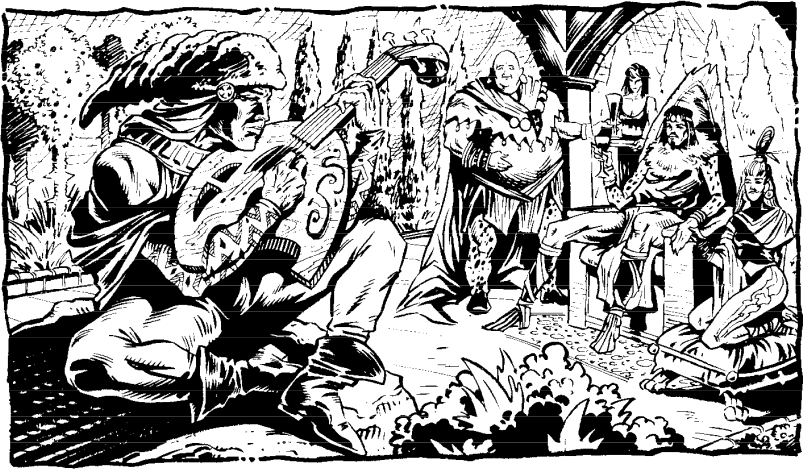
\includegraphics[width=\textwidth]{images/bard-2.png}
\par\textit{\small\textcopyright Wizards of the Coast, 2020.}
\end{figure*}

\textbf{Bardic Music:} Once per day per bard level, a bard can use his song or poetics to produce magical effects on those around him (usually including himself, if desired). While these abilities fall under the category of bardic music and the descriptions discuss singing or playing instruments, they can all be activated by reciting poetry, chanting, singing lyrical songs, singing melodies, whistling, playing an instrument, or playing an instrument in combination with some spoken performance. Each ability requires both a minimum bard level and a minimum number of ranks in the \skill{Perform} skill to qualify; if a bard does not have the required number of ranks in at least one \skill{Perform} skill, he does not gain the bardic music ability until he acquires the needed ranks.

Starting a bardic music effect is a standard action. Some bardic music abilities require concentration, which means the bard must take a standard action each round to maintain the ability. Even while using bardic music that doesn't require concentration, a bard cannot cast spells, activate magic items by spell completion (such as scrolls), spell trigger (such as wands), or command word. Just as for casting a spell with a verbal component, a deaf bard has a 20\% chance to fail when attempting to use bardic music. If he fails, the attempt still counts against his daily limit.

\textit{Countersong (Su):} A bard with 3 or more ranks in a \skill{Perform} skill can use his music or poetics to counter magical effects that depend on sound (but not spells that simply have verbal components). Each round of the countersong, he makes a \skill{Perform} check. Any creature within 9 meters of the bard (including the bard himself) that is affected by a sonic or language-dependent magical attack may use the bard's \skill{Perform} check result in place of its saving throw if, after the saving throw is rolled, the \skill{Perform} check result proves to be higher. If a creature within range of the countersong is already under the effect of a noninstantaneous sonic or language-dependent magical attack, it gains another saving throw against the effect each round it hears the countersong, but it must use the bard's \skill{Perform} check result for the save. Countersong has no effect against effects that don't allow saves. The bard may keep up the countersong for 10 rounds.

\textit{Fascinate (Sp):} A bard with 3 or more ranks in a \skill{Perform} skill can use his music or poetics to cause one or more creatures to become fascinated with him. Each creature to be fascinated must be within 27 meters, able to see and hear the bard, and able to pay attention to him. The bard must also be able to see the creature. The distraction of a nearby combat or other dangers prevents the ability from working. For every three levels a bard attains beyond 1st, he can target one additional creature with a single use of this ability.

To use the ability, a bard makes a \skill{Perform} check. His check result is the DC for each affected creature's Will save against the effect. If a creature's saving throw succeeds, the bard cannot attempt to fascinate that creature again for 24 hours. If its saving throw fails, the creature sits quietly and listens to the song, taking no other actions, for as long as the bard continues to play and concentrate (up to a maximum of 1 round per bard level). While fascinated, a target takes a $-4$ penalty on skill checks made as reactions, such as \skill{Listen} and \skill{Spot} checks. Any potential threat requires the bard to make another \skill{Perform} check and allows the creature a new saving throw against a DC equal to the new \skill{Perform} check result.

Any obvious threat, such as someone drawing a weapon, casting a spell, or aiming a ranged weapon at the target, automatically breaks the effect. Fascinate is an enchantment (compulsion), mind-affecting ability.

\textit{Inspire Courage (Su):} A bard with 3 or more ranks in a \skill{Perform} skill can use song or poetics to inspire courage in his allies (including himself), bolstering them against fear and improving their combat abilities. To be affected, an ally must be able to hear the bard sing. The effect lasts for as long as the ally hears the bard sing and for 5 rounds thereafter. An affected ally receives a +1 morale bonus on saving throws against charm and fear effects and a +1 morale bonus on attack and weapon damage rolls. At 8th level, and every six bard levels thereafter, this bonus increases by 1 (+2 at 8th, +3 at 14th, and +4 at 20th). Inspire courage is a mind-affecting ability.

\textit{Inspire Competence (Su):} A bard of 3rd level or higher with 6 or more ranks in a \skill{Perform} skill can use his music or poetics to help an ally succeed at a task. The ally must be within 9 meters and able to see and hear the bard. The bard must also be able to see the ally.

The ally gets a +2 competence bonus on skill checks with a particular skill as long as he or she continues to hear the bard's music. Certain uses of this ability are infeasible. The effect lasts as long as the bard concentrates, up to a maximum of 2 minutes. A bard can't inspire competence in himself. Inspire competence is a mind-affecting ability.

\textit{Suggestion (Sp):} A bard of 6th level or higher with 9 or more ranks in a \skill{Perform} skill can make a suggestion (as the spell) to a creature that he has already fascinated. Using this ability does not break the bard's concentration on the fascinate effect, nor does it allow a second saving throw against the fascinate effect.

Making a suggestion doesn't count against a bard's daily limit on bardic music \skill{perform}ances. A Will saving throw (DC 10 + \onehalf bard's level + bard's Cha modifier) negates the effect. This ability affects only a single creature (but see mass suggestion, below). Suggestion is an enchantment (compulsion), mind-affecting, language dependent ability.

\textit{Inspire Greatness (Su):} A bard of 9th level or higher with 12 or more ranks in a \skill{Perform} skill can use music or poetics to inspire greatness in himself or a single willing ally within 9 meters, granting him or her extra fighting capability. For every three levels a bard attains beyond 9th, he can target one additional ally with a single use of this ability (two at 12th level, three at 15th, four at 18th). To inspire greatness, a bard must sing and an ally must hear him sing. The effect lasts for as long as the ally hears the bard sing and for 5 rounds thereafter. A creature inspired with greatness gains 2 bonus Hit Dice (d10s), the commensurate number of temporary hit points (apply the target's Constitution modifier, if any, to these bonus Hit Dice), a +2 competence bonus on attack rolls, and a +1 competence bonus on Fortitude saves. The bonus Hit Dice count as regular Hit Dice for determining the effect of spells that are Hit Dice dependent. Inspire greatness is a mind-affecting ability.

\textit{Song of Freedom (Sp):} A bard of 12th level or higher with 15 or more ranks in a \skill{Perform} skill can use music or poetics to create an effect equivalent to the break enchantment spell (caster level equals the character's bard level). Using this ability requires 1 minute of uninterrupted concentration and music, and it functions on a single target within 9 meters. A bard can't use song of freedom on himself.

\textit{Inspire Heroics (Su):} A bard of 15th level or higher with 18 or more ranks in a \skill{Perform} skill can use music or poetics to inspire tremendous heroism in himself or a single willing ally within 9 meters. For every three bard levels the character attains beyond 15th, he can inspire heroics in one additional creature. To inspire heroics, a bard must sing and an ally must hear the bard sing for a full round. A creature so inspired gains a +4 morale bonus on saving throws and a +4 dodge bonus to AC. The effect lasts for as long as the ally hears the bard sing and for up to 5 rounds thereafter. Inspire heroics is a mind-affecting ability.

\textit{Mass Suggestion (Sp):} This ability functions like suggestion, above, except that a bard of 18th level or higher with 21 or more ranks in a \skill{Perform} skill can make the suggestion simultaneously to any number of creatures that he has already fascinated. Mass suggestion is an enchantment (compulsion), mind-affecting, language-dependent ability.

\textbf{Smuggler (Ex):} A bard receives a +1 insight bonus to \skill{Bluff} and \skill{Sleight of Hand} checks for every two bard levels.

\textbf{Poison Use:} Bards are trained in the use of poisons, and as of 2nd level, never risk accidentally poisoning themselves when applying poison to a blade.

\textbf{Streetsmart (Ex):} When a bard reaches 2nd level, he gets a +2 competence bonus to \skill{Gather Information} and \skill{Intimidate} checks.

\textbf{Quick Draw:} Bards learn to strike quickly and without warning. At 3rd level, a bard gains \feat{Quick Draw} as a bonus feat.

\textbf{Trade Secrets:} At every 4th level a bard learns a trade secret chosen from the list below.

\textit{Alchemy Dealer:} A bard with this trade secret pays one-half of the market price for raw materials needed to craft alchemical items.

\textit{Accurate:} When a bard with this trade secret attacks an armored opponent, his accuracy allows him to ignore 1 point of natural armor bonus to AC or 1 point of armor bonus to AC. This trade secret may be chosen more than once, and its effects stack.

\textit{Agile:} A bard with this trade secret receives a +1 dodge bonus to AC. This trade secret may be chosen more than once, and its effects stack.

\textit{Coolheaded:} A bard with this trade secret may take 10 on \skill{Bluff} and \skill{Diplomacy} checks.

\textit{Improvised Materials:} A bard with this trade secret can craft poisons from raw materials at hand instead of relying on specific ingredients. Doing so increases the \skill{Craft} (poisonmaking) check DC by 5 but otherwise has no effect on the poison's potency.

\textit{Poison Dealer:} A bard with this trade secret pays one-half of the market price for raw materials needed to craft poisons.

\textit{Poisonbane:} A bard with this trade secret receives a +4 insight bonus to \skill{Craft} (alchemy) checks when creating antitoxin and poison antidotes.

\textit{Poison Resistance:} A bard with this trade secret receives a +4 bonus to saving throws against poisons.

\textit{Scorpion's Touch:} A bard with this trade secret adds +1 to the save DC of all poisons applied by him. This trade secret may be chosen more than once, and its effects stack.

\textit{Skilled:} A bard with this trade secret adds one-half your bard level (rounded down) as a competence bonus to one of the following skills: \skill{Appraise}, \skill{Bluff}, \skill{Craft}, \skill{Diplomacy}, \skill{Heal}, \skill{Perform}, \skill{Profession}, \skill{Sense Motive} or \skill{Sleight of Hand}. This trade secret may be chosen more than once, each time it applies to a different skill.

\textit{Smokestick Application:} A bard with this trade secret can combine inhaled poisons with smokesticks. All creatures within the area the smokestick covers (10-ft. cube) are affected by the poison you applied to the smokestick.

\textit{Versatile:} A bard with this trade secret selects any two non-class skills to be considered class skills.

\textbf{Mental Resistance (Ex):} Bards carry many dark secrets they would prefer remain secret. This, combined with a large amount of knowledge based on half-truths and false rumors makes your mind unreliable to those who would seek to mentally affect it. A 5th level bard receives a +2 morale bonus to saves made against telepathic powers and enchantment/charm spells.

\textbf{Improved Poison Use (Ex):} At 6th level, a bard can apply poison to a weapon as a free action without provoking attacks of opportunity.

\textbf{Quick Thinking (Ex):} Bards often find themselves in a tight spot where they have to act quickly, whether it is to escape a templar patrol or strike first when in confrontation with a foe. At 6th level, a bard gets a +2 bonus on initiative checks. This bonus increases by 2 at 11th and 16th level.

\textbf{Chance (Ex):} Bards live on the edge in many ways. At 7th level, a bard may reroll one single d20 roll once per day, but have to keep the latter result---for better or for worse. At 14th level, a bard may use this ability two times per day.

\textbf{Speed Reactions (Ex):} Beginning at 9th level, when a bard uses the attack action or full attack action in melee, he may subtract a number from all melee attack rolls and add the same number to his initiative. This number may not exceed his base attack bonus. He may not make ranged attacks this round. The initiative increase takes effect on the next round. The new initiative is his initiative for the remainder of the combat, unless you were to use speed reactions again, which would increase your initiative further.

\textbf{Slippery Mind (Ex):} If a 10th level bard is affected by an enchantment spell or effect and fails her saving throw, she can attempt it again 1 round later at the same DC. She gets only this one extra chance to succeed on her saving throw.

\textbf{Defensive Roll (Ex):} At 15th level a bard learns how to avoid a potentially lethal blow to take less damage from it than you otherwise would. Once per day, when he would be reduced to 0 or fewer hit points by damage in combat (from a weapon or other blow, not a spell or special ability), the bard can attempt to roll with the damage. To use this ability, the bard must attempt a Reflex saving throw (DC = damage dealt). If the save succeeds, he takes only half damage from the blow; if it fails, he takes full damage. He must be aware of the attack and able to react to it in order to execute his defensive roll---if he is denied her Dexterity bonus to AC, he can't use this ability. Since this effect would not normally allow a character to make a Reflex save for half damage, the rogue's evasion ability does not apply to the defensive roll.

\textbf{Awareness (Ex):} At 17th level, you are never caught flat-footed and always act in the surprise round.

\textbf{Mind Blank (Sp):} At 18th level your mind becomes completely sealed against involuntary intrusion as per the mindblank spell. This spell-like ability is always considered active.

\subsection{Playing a Bard}

You are a master of oral tradition and lore, and a true artist, but you share your talents only with those who can afford to pay you.

You are an artist. You are the center of attention (whenever you want to), the person everyone wants to talk to, the ``face'' of the party. Even if you aren't the most attractive or charismatic member of your group, your unequaled skill at performance arts creates an irresistible appeal born of justified confidence. You are more than just light entertainment, though. Your target rarely survives the encounter if you don't want him to.

You might adventure because you desire entertainment. Someone with your smarts gets bored easily. Alternatively, you may have been blacklisted on your current location because of a ``business transaction'' gone wrong. You have to keep moving, and adventuring offers you a regular change of scenery. In any case, a life of adventure allows you to see new things, meet interesting people, and get some silvers in the process.

\subsubsection{Religion}

No central bardic organization exists, and more often than not bards have no particular penchant for religion. Some may worship the elements, fearing the power of the elemental forces, and most bards tend to relate to the Air ever-changing nature, but bards that worship sorcerer-kings are rare. A lifestyle of breaking the rules of the city-states does not lend one to worship the lawgivers.

\subsubsection{Other Classes}

Bards face life as it comes, and usually hold no special grudge or awe for any one class. They usually approach other's profession on the basis of how it can help them at the moment. Clerics and druids are respected for their devotion to a divine force, but usually not held in awe. Fighters, gladiators and rangers can be useful as sword-arms but are otherwise useless to the bard. Bards do not view wizards with the same aversion as others might view them, since bards sell them their components.

\subsubsection{Combat}

A bard rarely seeks to initiate combat---instead he skulks about, looking for an opportunity to strike swiftly, using his poisons to their greatest advantage. Your work best with teammates, maneuvering to get flanks and help bring down opponents with your various poisons. Use your bardic music to bolster your allies and distract your opponents while the real heavy hitters in your group mop them up.

\subsubsection{Advancement}

You have a flexibility in building your talents unrivaled by any other class. You can either emphasize on ability or nurse a broad range of abilities. In most cases, feats that consistently improve your talents are more useful than feats that function in only certain situations.

As you advance in the class, continue to max out your ranks in Bluff and Perform, and invest skill points in Gather Information and Sleight of Hand. Many feats in the Athasian Emporium supplement make the most of your poison abilities. Improved Feint is an excellent choice with your expertise in Bluff, and Greasing the Wheels (page 72) if perfect for getting around templar inspections. If you play up the assassin aspect of this class, consider magic (or psionic) items that help you cloak your true intentions, such as an amulet of proof against detection and location or a veil of lies (page 260).

When multiclassing or taking a level in a prestige class, find combinations that further broaden your abilities or that increase your flexibility. The poisonmaster prestige class (page 101), the dune trader (page 90), and the assassin (DMG 180) deserve special mention. They are a great combination with the bard class.

\subsection{Starting Packages}
\subsubsection{The Assassin}
Elf Bard

\textbf{Ability Scores:} Str 13, Dex 17, Con 10, Int 10, Wis 14, Cha 8.

\textbf{Skills:} \skill{Climb}, \skill{Disguise}, \skill{Hide}, \skill{Move Silently}, \skill{Open Lock}, \skill{Spot}.

\textbf{Languages:} Elven, Common.

\textbf{Feat:} \feat{Stealthy}.

\textbf{Weapons:} Bard's friend (1d4/18-20)

Shortbow with 20 arrows (1d6/$\times$3, 18 m).

\textbf{Armor:} Studded leather (+3 AC).

\textbf{Gear:} Standard adventurer's kit, thieves' tools, musical instrument, 9 cp.

\subsubsection{The Information Smuggler}
Human Bard

\textbf{Ability Scores:} Str 8, Dex, 12, Con 10, Int 15, Wis 14, Cha 13.

\textbf{Skills:} \skill{Bluff}, \skill{Decipher Script}, \skill{Diplomacy}, \skill{Gather Information}, \skill{Knowledge} (local), \skill{Listen}, \skill{Sense Motive}.

\textbf{Languages:} City language, Common, Elven.

\textbf{Feat:} \feat{Investigator}, \feat{Negotiator}.

\textbf{Weapons:} Widow's knife (1d4/$\times$3)

Light crossbow with 20 bolts (1d8/19-20, 24 m).

\textbf{Armor:} Leather armor (+2 AC).

\textbf{Gear:} Standard adventurer's kit, 4 cp.

\subsubsection{The Poisoner}
Half-elf Bard

\textbf{Ability Scores:} Str 8, Dex 15, Con 10, Int 15, Wis 14, Cha 6.

\textbf{Skills:} \skill{Appraise}, \skill{Craft} (alchemy), \skill{Craft} (poisonmaking), \skill{Knowledge} (local), \skill{Sleight of Hand}.

\textbf{Languages:} City language, Common, Elven.

\textbf{Feat:} \feat{Skill Focus} (Craft [poisonmaking]).

\textbf{Weapons:} Bard's friend (1d4/18-20)

Blowgun with 20 needles (1, 3 m).

\textbf{Armor:} Shell armor (+4 AC).

\textbf{Gear:} Standard adventurer's kit, smokestick, 4 cp.

\subsection{Bards on Athas}
\Quote{She was a rare beauty: charming, graceful, talented. It's too bad she killed my boss.}{Talos, mul bodyguard}

Athasian bards use songs and tales as their tools of trade. A bard is a person of wit and camaraderie. Despite having few other talents to offer, the bard is a welcome source of entertainment and information across Athas. However, bards are noted to be extremely untrustworthy and even ruthless---they often sell their skills as assassins and poison alchemists to the highest bidder.

In the cities, bards often become tools of the nobility. They're commonly hired by one noble house and sent to another as a gift. The bards are sent not only to entertain, but usually to perform some other subtle task as well (such as robbery, espionage, or even assassination).

Nobles consider it rude to turn down the gift of a bard or bard company. However, when presented with a troop of bards from one's worst enemy, it's sometimes better to be rude and turn them away, for the consequences of their visit could be downright deadly. To get around this, the noble who hired them sometimes disguises their approach by having another noble send them. A very complicated collage of intrigue and deceit is often woven wherever bards are involved.

\subsubsection{Daily Life}

The way a bard behaves depends on his individual sense of morality. Some think nothing of adopting false identities, smuggling forbidden goods, or even coldblooded assassination. Other bards find themselves driven to use their skills to entertain and help people.

Bards can become great leaders. With their quick wits and great charisma, bards would be natural leaders were it not for their inconstancy. If a bard manages to earn the trust of companions, they value his leadership. Lacking that trust, a bard rarely leads for long.

\subsubsection{Notables}

Bards often gain notoriety for their deeds, although most prefer to remain behind false identities. The human bard only known as Wheelock has become a legend when it comes to creating poisons. Fyrian Wynder is a Tyrian half-elven bard notorious for his combination of bardic abilities and the Way, since his acting skills enable him to adopt several identities, while his psionic abilities provide a means of gaining access to secured areas and going unnoticed once he gets there.

\subsubsection{Organizations}

Bards don't organize together, but they often linger around the same places, which end up getting known as the Bard's Quarter in most city-states. A bard joining an organization probably has a specific goal (or target) in mind and rakes a position that best allows him to attain it. A long-term commitment to such a group rarely appeals to a bard.

\subsubsection{NPC Reactions}

Common folk ten to have a hard time differentiating bards from rogues. Bards further confuse the issue by regularly adopting false identities and hiding their varied abilities. Thus, the reaction a bard gets from those he meets depends on what he is pretending to be at a time. Individuals who know about the bard class and the reputation that comes with it have an initial attitude one step more hostile than normal. Templars in particular look poorly upon bards, since they know of the various illegal activities they usually perform.

\subsubsection{Bard Lore}

Characters with ranks in \skill{Knowledge} (local) can research bards to learn more about them. When a character makes a skill check, read or paraphrase the following, including the information from lower DCs.

\textbf{DC 15:} Bards are jacks of all trades, masters of performance and deception, and information smugglers.

\textbf{DC 20:} Bards are masters of poisons and lore, and they have many of the skills of rogues.